% ============================================================
% 4. RISK MANAGEMENT PLAN
% ============================================================
\clearpage
\section{Risk Management Plan}

\subsection{Risk management approach}
\subsubsection{Risk identification methodology}
\placeholder{Insert methodology.}

\subsubsection{Risk assessment criteria and scales}
\placeholder{Define probability, impact, scoring, and rating thresholds.}

\subsubsection{Risk monitoring and control process}
\placeholder{Insert monitoring and control process.}

\subsubsection{Risk reporting frequency and format}
\placeholder{Insert reporting process.}

\subsubsection{Risk escalation thresholds}
\placeholder{Insert escalation thresholds.}

\subsection{Risk register}
% The Skeleton requires at least 12 risks.
% This table is intentionally placed on landscape pages in the final document
% if portrait layout makes the response-action column difficult to read.
% Recommended columns: Risk ID, Description, Category, Probability, Impact,
% Score, Response strategy, Specific response action, Owner, Trigger conditions.
\placeholder{Insert risk register with at least 12 risks.}

\subsection{Probability/impact matrix}
\begin{figure}[H]
  \centering
  \IfFileExists{figures/meridian_risk_matrix.pdf}{%
    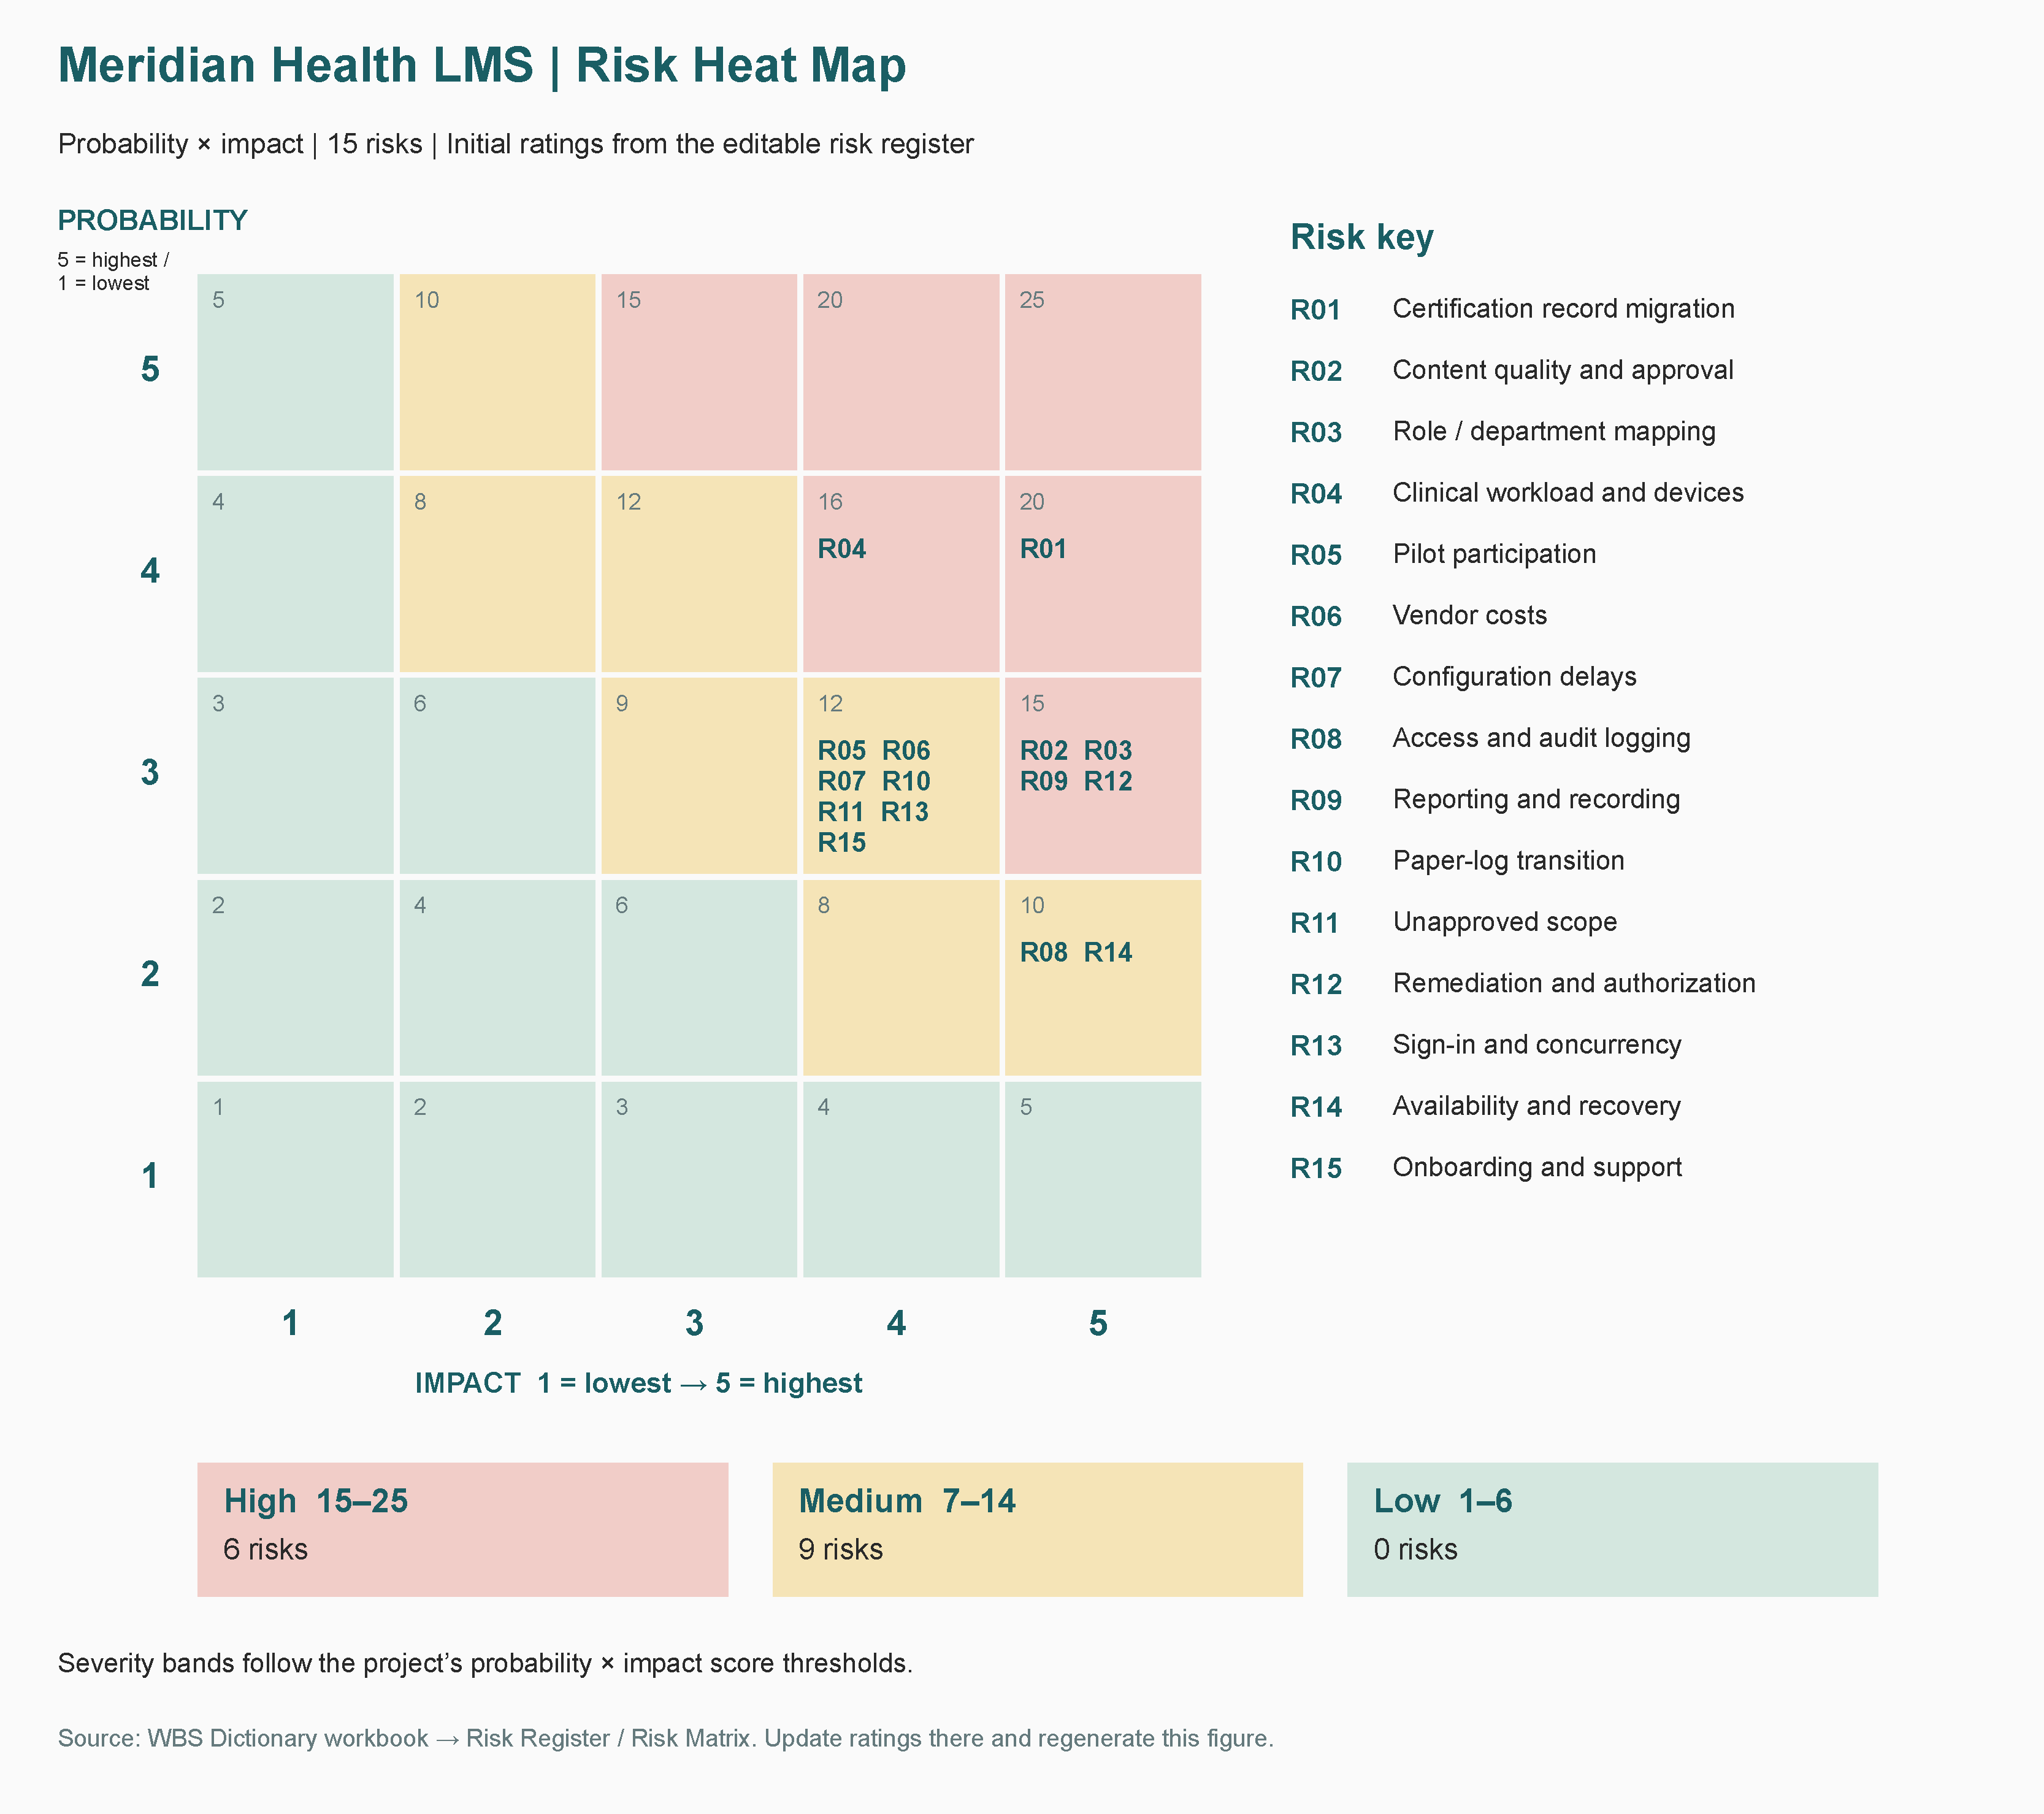
\includegraphics[width=0.78\textwidth,height=0.58\textheight,keepaspectratio]{figures/meridian_risk_matrix.pdf}%
  }{\fbox{\parbox[c][1.5in][c]{0.75\textwidth}{\centering
    Risk matrix placeholder. Upload \texttt{figures/meridian\_risk\_matrix.pdf}.}}}
  \caption{Probability/impact matrix for the Meridian Health LMS project.}
  \label{fig:risk-matrix}
\end{figure}
